\pagenumbering{arabic}
\section{绪论}
\subsection{研究背景}
在固体物理中,重费米子材料是一种特殊的过渡金属化合物属于强关联电子系统如\ce{Ce3PtIn11}。重费米子化合物的性质通常来自稀土或锕系元素离子的部分填充的f轨道,表现为有效的局域磁矩。“重费米子”这个名字来自于费米子的行为,即它的有效质量大于其静止质量。以电子为例,低于特征温度时(通常为10$K$),这些金属化合物中的传导电子表现为它们的有效质量是自由粒子质量的100到1000倍。

重费米子材料由K.Andres,J.E.Graebner和H.R.Ott在1975年发现,他们观察到\ce{CeAl3}中线性比热容变化很大,在对掺杂超导体的研究中得出结论:一种材料中存在局域磁矩和超导态是不相容的,但是在1979年。Frank Steglich等人在\ce{CeCu2Si2}中发现了重费米子的超导性。H.von Löhneysen等人于1994年在重费米子化合物的相图中发现了量子临界点和非费米液体行为,导致人们对这些化合物的研究产生了新的兴趣。另一个实验突破是(由Gil Lonzarich小组证明)重费米子中的量子临界性可能是非常规超导性的原因。


本文目的是利用Determinant Quantum Monte Carlo(DQMC),构建对这类材料的有效模型,针对构建的模型进行计算模拟研究,对\ce{Ce3(Pd/Pt)In11}材料中发现的超导与反铁磁共存的现象进行模拟。






\subsection{理论模型}

\subsubsection{Hubbard模型}
在一般的固体理论中,一般是将电子与电子之间的相互作用忽略,只考虑泡利不相容原理,故系统哈密顿量不存在电子相互作用。但是在实际中,尤其是窄能带晶体中,电子之间的相互作用无法忽略,如过渡金属氧化物和镧系氧化物,前者3d轨道之间交叠很大,d轨道上的电子相互作用无法忽略,把这部分相互作用写入哈密顿量就得到了强关联模型即Hubbard模型\cite{1}。

多体系统的总哈密顿量为
\begin{align*}
    H&=\sum_i h(\textbf{r}_i)+\frac{1}{2}\sum_{i,j}v_{ij}\\
    v_{ij}&=\frac{e^2}{|\textbf{r}_i-\textbf{r}_j|}
\end{align*}

只考虑单个未填满的能带,如孤立的s带,在布洛赫表象中考虑相互作用哈密顿量二次量化表示式可写成
\begin{equation}
    H=\sum_{k, \sigma} E_{k} C_{k \sigma}^{+} C_{k \sigma}+\frac{1}{2} \sum_{k_{1}, k_{2}, k_{1}^{\prime}, k_{2}^{\prime}} \sum_{\sigma, \sigma^{\prime}}<k_{1}, k_{2}|v| k_{1}^{\prime}, k_{2}^{\prime}>C_{k_{1} \sigma}^{+} C_{k_{2} \sigma^{\prime}}^{+} C_{k^{\prime}_2 \sigma^{\prime}} C_{k^{\prime}_1 \sigma}
    \label{1.1}
\end{equation}

其中$E_k$是能带电子的能量,$C^+_{k \sigma}$和$C_{k \sigma}$代表布洛赫轨道上$\sigma$自旋电子的产生及湮灭算符。

我们采用Wannier表象
\begin{align*}
    \psi_k(\textbf{r})&=N^{-\frac{1}{2}}\sum_i e^{i\textbf{k}\cdot \textbf{R}_i} a(\textbf{k} - \textbf{R}_i)\\
    C^+_{i \sigma}&=N^{-\frac{1}{2}} \sum_k e^{- i\textbf{k}\cdot \textbf{R}_i} C^+_{k \sigma}\\
    C_{i \sigma}&=N^{-\frac{1}{2}} \sum_k e^{i\textbf{k}\cdot \textbf{R}_i} C_{k \sigma}
\end{align*}
将\ref{1.1}式变换为
$$
H=\sum_{i, j} \sum_{\sigma} T_{i j} C_{i \sigma}^{+} C_{j \sigma}+\frac{1}{2} \sum_{i, j, l, m} \sum_{\sigma, \sigma^{\prime}}<i j|v| l m>C_{i \sigma}^{+} C_{j \sigma^{\prime}}^{+} C_{m \sigma^{\prime}} C_{l \sigma}
$$
其中
$$T_{ij}=N^{-1}\sum_k e^{i \textbf{k} \cdot (\textbf{R}_i-\textbf{R}_j)}\textbf{E}_k$$
对于窄带单中心积分
$$
<i i|v| i i>\equiv U=e^{2} \int \frac{a^{*}\left(r-R_{i}\right) a^{*}\left(r^{\prime}-R_{i}\right) a\left(r-R_{i}\right) a\left(r^{\prime}-R_{i}\right)}{\left|r-r^{\prime}\right|} \mathrm{d} r \mathrm{~d} r^{\prime}
$$
是最重要的,代表同一格点周围能带电子之间的库伦作用。作为一个简单的模型,可以略去相互作用项中所有的多中心积分,只取单中心积分项。可以得到Hubbard哈密顿量
$$
H=\sum_{i, j} \sum_{\sigma} T_{i j} C_{i \sigma}^{+} C_{j \sigma}+\frac{U}{2} \sum_{i} \sum_{\sigma} n_{i \sigma} n_{i \sigma}^{-}
$$

\subsubsection{周期安德森模型}
周期安德森模型是 P. W. Anderson提出用哈密顿量解决金属中的磁性杂质\cite{2}。现用于描述近藤效应的问题,例如重费米子系统以及近藤绝缘体。对于单个杂质,哈密顿量为
$$
H=\sum_{k, \sigma} \epsilon_{k} c_{k \sigma}^{\dagger} c_{k \sigma}+\sum_{\sigma} \epsilon_{d} d_{\sigma}^{\dagger} d_{\sigma}+U d_{\uparrow}^{\dagger} d_{\uparrow} d_{\downarrow}^{\dagger} d_{\downarrow}+\sum_{k, \sigma} V_{k}\left(d_{\sigma}^{\dagger} c_{k \sigma}+c_{k \sigma}^{\dagger} d_{\sigma}\right)
$$
其中c是传导电子的湮灭算符,d是杂质的湮灭算符,k是传导电子波矢量,$\sigma$标记自旋,U是库伦排斥,V表示杂化。

对于重费米子系统,周期安德森模型(PAM)描述了杂质晶格,其中一维模型哈密顿量为
$$
H=\sum_{k, \sigma} \epsilon_{k} c_{k \sigma}^{\dagger} c_{k \sigma}+\sum_{j, \sigma} \epsilon_{f} f_{j \sigma}^{\dagger} f_{j \sigma}+U \sum_{j} f_{j \uparrow}^{\dagger} f_{j \uparrow} f_{j \downarrow}^{\dagger} f_{j \downarrow}+\sum_{j, k, \sigma} V_{j k}\left(e^{i k x_{j}} f_{j \sigma}^{\dagger} c_{k \sigma}+e^{-i k x_{j}} c_{k \sigma}^{\dagger} f_{j \sigma}\right)
$$
其中$x_j$是杂质位点j的位置,f是杂质产生算符(在重费米子系统中按照惯例用d代替),杂化项允许重费米子系统中的f轨道的电子相互作用,即使电子之间最大距离超过了Hill极限(Hill极限是锕系元素或稀土原子晶格中定义的临界距离,即晶格中的两个原子如果相隔的距离大于Hill极限,f轨道的重叠就可以忽略不计)。%解释Hill极限

\subsubsection{Kondo效应}
近藤效应描述了金属中传导电子由于磁性杂质的散射,从而导致特性变化,即电阻率随温度变化的最小值(如图\ref{fig})。近藤俊彦首先解释了这种影响的原因\cite{3},他将三阶微扰理论应用于该问题,以解释s轨道传导电子对杂质处d轨道电子的散射(近藤模型)。
\begin{figure}[h]
    \centering
    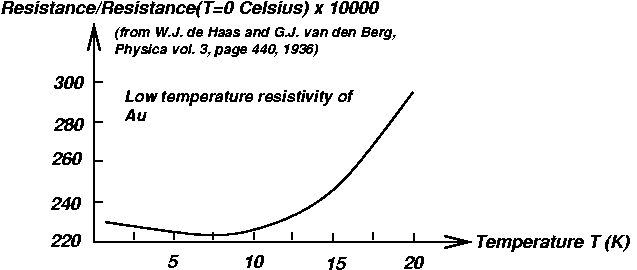
\includegraphics[scale=0.6]{/mnt/d/共享文件夹/毕设论文/latex模板/figures/Classickondo.png}
    \caption{含有少量铁杂质的金在低温下的行为\cite{4}。}
    \label{fig}
\end{figure}
电阻率$\rho$在考虑了近藤效应后对温度T的依赖关系,如下
$$
\rho(T)=\rho_{0}+a T^{2}+c_{m} \ln \frac{\mu}{T}+b T^{5}
$$
其中$\rho_0$表示剩余电阻率,$aT^2$表示费米液体性质的贡献,$bT^5$表示晶格振动:$a,b,c_m$和$\mu$是与温度无关的量。近藤俊彦导出了第三项,该项与温度和实验观察到的呈对数关系。


\subsubsection{Ruderman–Kittel–Kasuya–Yosida(RKKY)相互作用}
RKKY interaction指的是通过传导电子的相互作用,金属中的核磁矩或局域内部d或f壳层电子自旋的耦合机制\cite{5}\cite{6}\cite{7}。

RKKY相互作用最初由加州大学伯克利分校的马尔文·鲁德曼(Malvin Ruderman)和查尔斯·基特尔(Charles Kittel)提出,作为一种解释在天然金属银中观察到的异常宽的核自旋共振线的方法。该理论使用二阶微扰理论来描述间接交换耦合,其中一个原子的核自旋通过超精细相互作用与传导电子相互作用,该传导电子与另一个核自旋相互作用,从而在两个核自旋之间产生关联能。(与核自旋通过超精细相互作用耦合到传导自旋不同,另一种情况是内部电子自旋通过交换相互作用耦合到传导自旋。)该理论基于布洛赫波函数,因此仅适用于晶体系统。派生的相互作用采用以下形式:
$$
H\left(\mathbf{R}_{i j}\right)=\frac{\mathbf{I}_{i} \cdot \mathbf{I}_{j}}{4} \frac{\left|\Delta_{k_{m} k_{m}}\right|^{2} m^{*}}{(2 \pi)^{3} R_{i j}^{4} \hbar^2}\left[2 k_{m} R_{i j} \cos \left(2 k_{m} R_{i j}\right)-\sin \left(2 k_{m} R_{i j}\right)\right]
$$
其中H代表了哈密顿量,$R_{i,j}$代表了i和j两原子核之间的距离,$\mathbf{I}_i$为原子i的核自旋,$\Delta_{k_{m}k_m}$表示超精细相互作用强度的矩阵元,$m^*$表示晶格中的电子的有效质量,$k_m$是费米动量。 







\section{\ce{Ce3(Pt/Pd)In11}重费米子物理体系}
\subsection{概述}
迄今为止研究的大多数铈重费米子化合物都有 一个Ce离子的晶体学位点。在两个或者更多不等位点的化合物中,相应Ce离子的不同的局部环境导致Ce的4f轨道态与周围的配合基和传导态的不同相互 作用。这反过来导致不同的近藤耦合强度。因此,在这些多位点铈化合物中,可能会出现各种新的和复杂的现象,其中基态的特征在于不同电子和磁性状态在微观尺度上的共存。如图\ref{fig1},\ce{Ce3PdIn11}拥有两个Ce不等位点,其中一个Ce位点表示出顺磁性($T_N \approx 0.3K$)而另一个Ce位点展现反铁磁性($T_Q \approx 0.5K$)。

\begin{figure}[h]
    \centering
    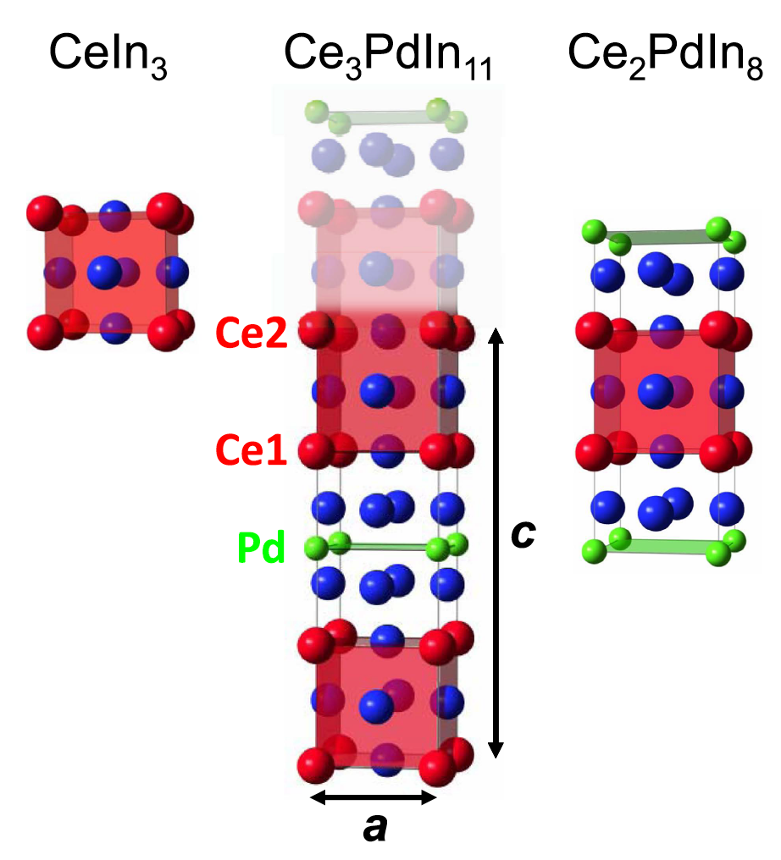
\includegraphics[scale=0.6]{/mnt/d/共享文件夹/毕设论文/latex模板/figures/figure 1.png}
    \caption{\Songti \ce{Ce3PdIn11}的晶格结构(中间),指出了Ce两个不等位点Ce1和Ce2\cite{8}。}%引用
    \label{fig1}
\end{figure}


\ce{Ce3PdIn11}和\ce{Ce3PtIn11}都属于\ce{Ce_nT_mIn_{3n+2m}}类材料。包括了\ce{CeCoIn5}、\ce{CeRhIn8}和\ce{Ce2\\RhIn8}等一系列化合物。\ce{Ce3PdIn11}和\ce{Ce3PtIn11}晶体结构相似。在室温下的晶格常数分别是$a=4.687(4)$\AA 和$c=16.8422(12)$\AA。

同样\ce{Ce3PtIn11}也拥有两个不等位点,晶胞中的三个Ce离子分布在晶体学上不等价的位点内。两个Ce离子位于Ce1的位置,其被类似于\ce{Ce2PtIn8}中的Ce离子的配体包围。Ce2的位置被一个Ce离子占据,离子拥有类似\ce{CeIn3}的环境。在无磁场的情况下,\ce{Ce3PtIn11}在$T_1 \simeq 2.2K$和$T_N \simeq 2K$处经历两次连续的变化,进入反铁磁状态(AFM),并在$T_c \simeq 0.32K$以下变为超导。

\subsection{物理性质}
\subsubsection{电阻率}
如图\ref{fig2}在300K时,c轴电阻率等于$600 \Omega cm$,大约是基平面$\rho$的1.5倍。随着温度降低$\rho$表现出随温度$d \rho /d t > 0$的弱相关性。低于30K电阻率下降很快标志着高温下的不连续近藤散射向低温下的重电子布洛赫态的变化的交叉点。

\begin{figure}[h]
    \centering
    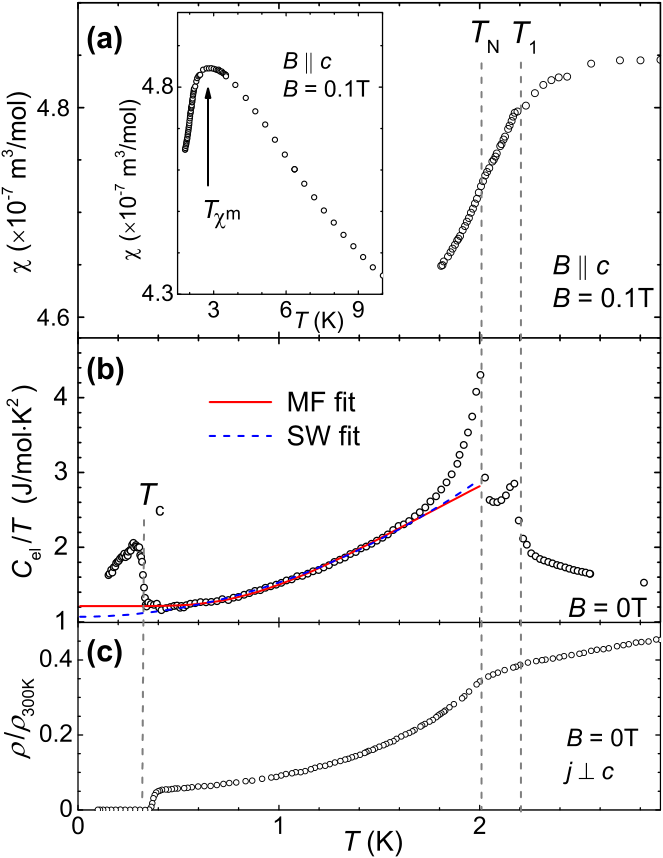
\includegraphics[scale=0.4]{/mnt/d/共享文件夹/毕设论文/latex模板/figures/figure4.png}
    \caption{\ce{Ce3PtIn11}在$T < 3K$时的低温 特性。(a)在施加于c轴$B = 0.1T$的磁场中$\chi$与T的相关性。插入的部分显示了温度数据最大是10K。箭头指出了$\chi T$的最大值。(b)电子部分的比热$C_el/T$作为T的函数在零场中。红色的实线和蓝色的虚线分 别是$T < 0.8T_N$到$T = 0$的一个均值场和自旋波的拟合。(c)电阻归一化到其室温的值在B=0T和$j\perp c$\cite{8}。}
    \label{fig2}
\end{figure}

\subsubsection{磁化系数}
$\chi(T)$沿晶格c轴和垂直于晶格c轴的磁场中测量到具有弱各向异性,在温度为3K时$\chi^{\parallel c}/\chi^{\perp c} \approx 1.25$。在超过150K时$\chi(T)$遵循Curie-Weiss定律两个方向的有效磁矩为$\mu_{eff}=2.60\mu_B /Ce$,与洪特规则对自由\ce{Ce^{3+}}离子符合很好。Weiss温度由对$\theta^{\perp c}_{p}=-64K$和$\theta^{\parallel c}_p=-42K$的曲线拟合到。图\ref{fig2}显示了\ce{Ce3PtIn11}在低温下的环境压力热力学和传输特性。在图\ref{fig2}(a)插入显示了在一个大的温度范围低温下磁化率$\chi^{\parallel c}$。

\subsubsection{反铁磁和非常规超导}
图\ref{fig2}(a)在更低温下$\chi(T)$在$T_1$时急剧下降,第二个AFM转变在$T \simeq 2.0k$表现为0.1T数据中显示为弱凸状结构。

将$C_{el}/T$跳跃的重点定义为过渡温度,分别得到$T_1 \simeq 2.2K$和$T_N \simeq 2K$,这些值与$\chi(T)$和$\rho(T)$的特征符合的很好(图\ref{fig2}中的虚线)。当$T=0.35K$时$C_{el}/T$发生了明显的变化,这表示了电阻率数据证实了材料向超导相的转变。将这个跳跃中点定义为$T_c \simeq 0.32K$。

为了估算通常比热系数$\gamma_n$外推AFM低温向$T=0$变化的尾部图\ref{fig2}b红色虚线部分采用二阶平均场类型表达式,$C_{el}/T=\gamma_n + A e^{-\Delta_{AFM}/T}$。拟合结果是$\gamma_n=1.21J/(molK^2)$,$A=8.97J/(molK^2)$和$\Delta_{AFM}=3.44K$(拟合区间是$0.44<T<1.6K$)。拟合$C_{el}/T \propto T^2$(AFM自旋波)描述了相同区间的数据,具有相似的质量,但是$\gamma_n$减小了大约10\%。使用上述参数可以计算参数$\Delta C/(\gamma T_c)\approx 0.7$,大约是BCS理论预期值的一半。我们可以在这里假设,参与超导的导带中的电子等量得来自两个Ce位点。







\section{反铁磁性和非常规超导共存和竞争机制}%分别介绍
\subsection{非常规超导简介}
在极低温下一些材料表现出完全抗磁性以及零电阻情况,常规超导可以用\\Bardeen-Cooper-Schrieffer (BCS)理论解释其中的微观图像:电子形成库伯对,配对电子可以凝聚,形成一个相位相干的宏观量子态。常规超导的共性:(1)常规材料的电子声子耦合较弱,转变温度$T_c$比较低;(2)超导态的序参量(超导电流密度)的对称性和晶格保持一致。常规超导体有广泛的应用前景,但是受限于较低转变温度$T_c$,难以大范围应用。

对非常规超导尤其是重费米子超导体的研究表明,电子确实可以通过多种关联效应引起的临界涨落配对,比如自旋涨落、电荷密度涨落、价态涨落等。这些涨落足够强时,可以像声子一样在电子对之间产生净吸引效应,而克服电子之间的库伦排斥力并产生超导现象。并且大量的实验数据证实,无论是从能量尺度还是对称性角度,非常规超导和量子相变往往是紧密联系的。
\subsection{超导与反铁磁的竞争与共存}
如图\ref{fig3}所示,重费米子超导的一个重要研究价值在其丰富的相图。图\ref{fig3}(c)表示,大部分材料的低温相图与铜氧化合物、铁基高温超导体又非常类似。但是最早发现Ce基超导的\ce{CeCu2Si2}仍然存在争议,从其相图看,材料中的超导和反铁磁序是竞争关系而非共存。可以简单理解为Ce原子的仅有的一个f电子很难同时参与反铁磁长程有序和超导序,但是并不妨碍反铁磁涨落与超导的共存关系。

2011年O.Stockert等人通过非弹性中子散射实验给出了反铁磁涨落驱动\ce{CeCu2Si2}超导的明确证据。在超导态,自旋激发能谱中看到了清晰的能隙,是由于磁交换能部分转变成了库伯对的凝聚能。同时在\ce{CeCu2Si2}、\ce{CePd2Si2}、\ce{CeAu2Si2}等材料都在高压下、反铁磁消失的边界区域出现超导相,暗示了超导与反铁磁相的竞争关系。



\begin{figure}[h]
    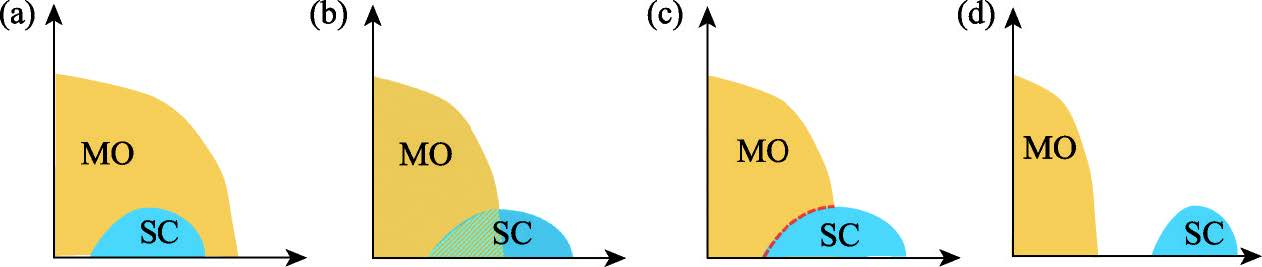
\includegraphics[scale=1.3]{/mnt/d/共享文件夹/毕设论文/latex模板/figures/figure5.jpg}
    \caption{重费米子超导体中超导相(SC)与磁有序相(MO)的竞争/共存相图,横坐标为化学掺 杂/替代、压力、偏压等调控手段,纵坐标为温度。(a)代表超导态完全处于磁有序相内 部,如 \ce{UGe2},\ce{YbRh2Si2} 等;(b)和(c)代表超导相从磁有序区域延伸到无磁性区域,但是(b)中超导与磁性可以在微观共存,如 \ce{CeRhIn5}、\ce{CePt3Si}、\ce{URhGe}、\ce{UCoGe}、(Ba,K)\ce{Fe2As2}等,而很多的 Ce 基、铜氧化合物、铁基超导体的相图与(c)一致;(d)代表 远离磁有序相以后材料才会出现超导态,比如 Pu-基超导体、\ce{CeCu2Si2}的高压超导相、\ce{\beta-YbAlB4} 等,价态涨落可能与这些材料的超导有关\cite{9}。}
    \label{fig3}
\end{figure}

在2000年前后,发现的\ce{CeMIn5}(M=Co,Rh,Ir)极大的拓展了我们对重费米子超导以及反铁磁量子临界行为的认识。它们化学性质的特点在于Co、Rh、Ir这三种元素可以互相替代,获得连续可调的反铁磁态和超导态,同时超导和反铁磁相可以在微观共存。在\ce{CeRhIn5}中,电子的自旋和电荷自由度通过Kondo效应和RKKY相互作用紧密联系在一起,在图\ref{fig4}中可以明显看到温度-压力-磁场相图中很好的反应出来。
\begin{figure}[h]
    \centering
    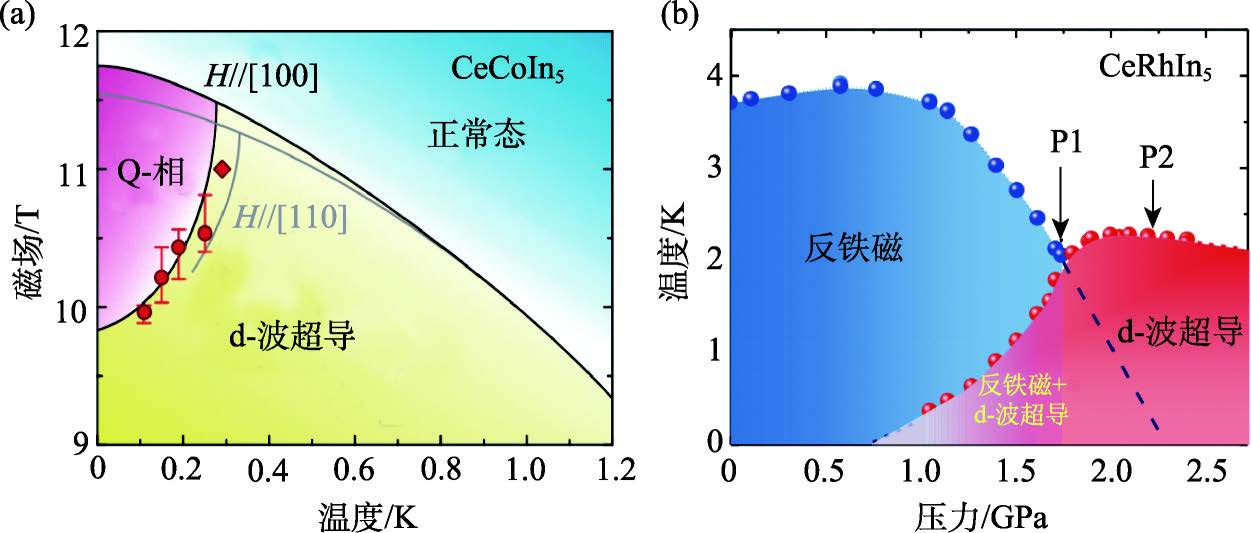
\includegraphics[scale=1]{/mnt/d/共享文件夹/毕设论文/latex模板/figures/figure6.jpg}
    \caption{(a)\ce{CeCoIn5}磁场温度相图,高磁场下粉红色区域为Q-相;(b)\ce{CeCoIn5}的压力-温度相图,中间粉色区域为超导与反铁磁共存的相\cite{9}。}
    \label{fig4}
\end{figure}









\section{关于\ce{Ce3PtIn11}的计算模拟研究}
\subsection{模型构建}
\subsubsection{哈密顿量}
为了阐述我们的发现,我们采用了最简化的原始模型如图\ref{fig4.1.1},该模型由两个不同的局域$f$轨道以及二维方形晶格上的传导电子组成:
\begin{eqnarray}
    {\cal H} &=& - t \sum\limits_{\langle ij \rangle \sigma}
(c^{\dagger}_{mi\sigma}c_{mj\sigma}^{\vphantom{dagger}}
+c^{\dagger}_{mj\sigma}c_{mi\sigma}^{\vphantom{dagger}})
- \mu \sum\limits_{i\sigma} (n^{c_m}_{i\sigma}+ n^{f_m}_{i\sigma} )  \nonumber \\
&+& V_m \sum\limits_{i \sigma}  (c^{\dagger}_{mi\sigma}f_{mi\sigma}^{\vphantom{dagger}}+ f^{\dagger}_{mi\sigma}c_{mi\sigma}^{\vphantom{dagger}}) \nonumber \\
 &+& V_{12} \sum\limits_{i \sigma}  (c^{\dagger}_{2i\sigma}f_{1i\sigma}^{\vphantom{dagger}}+ f^{\dagger}_{1i\sigma}c_{2i\sigma}^{\vphantom{dagger}}) \nonumber \\
    &+& U \sum\limits_{mi} (n^{f_m}_{i\uparrow}-\frac{1}{2}) (n^{f_m}_{i\downarrow}-\frac{1}{2})
\nonumber
\end{eqnarray}
式中,$c^{\dagger}_{i\sigma}(c_{i\sigma}^{\vphantom{dagger}})$和$f^{\dagger}_{mi\sigma}(f_{mi\sigma}^{\vphantom{dagger}})$与$m=1,2$是传导电子的产生(湮灭)算符和两个自旋为$i$的局域$f_{1,2}$电子。$n^{c,f_m}_{i\sigma}$是相关的数字运算符。最近邻位点$\langle ij \rangle$上的传导电子之间的跃迁$t=1$设置了能量标度。$U$是$f_{1,2}$轨道中的局域排斥相互作用。请注意,在这项工作中,为了简单起见,我们只考虑 $f_{1,2}$ 轨道拥有相同 $U$ 的情况,尽管它们通常可以不同。剩下的两个控制参数是两个不同的杂化,即 $c$-$f_1$ 之间的 $V$ 和 $c_2$-$f_1$ 之间的 $V_{12}$。
\begin{figure}[h]
    \centering
    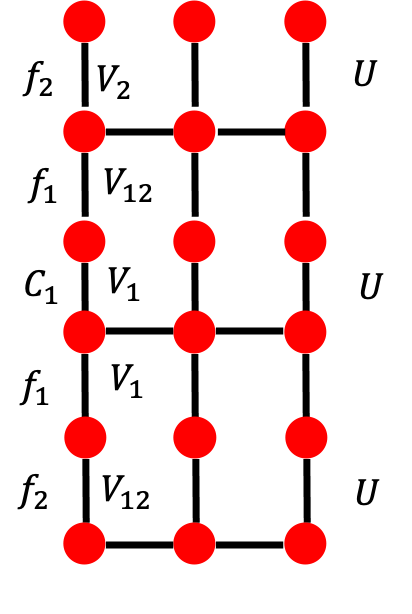
\includegraphics[scale=0.7]{/mnt/d/共享文件夹/毕设论文/latex模板/figures/figure2.png}
    \caption{\ce{Ce3PtIn11}的有效模型示意图,$V_2$和$V_{12}$以及$V_1$为两者间的跃迁能,$U$为局域排斥相互作用。}
    \label{fig4.1.1}
\end{figure}

\subsubsection{参数}
本文假设$V_1 \geqslant V_2$并主要关注有代表性的$f$轨道的Hubbard相互作用$U=4.0t$。此外,我们将传导轨道和f轨道都视为晶格位置,因此密度$\rho$实际上是两个轨道的平均密度。由于利用量子蒙特卡洛模拟这类费米子模型出现的符号问题并且兼顾到模拟时间的限制,在大多数情况下,本文使用较小的晶格尺寸如$4 \times 4$和$6 \times 6$,以便研究系统在低温下的行为。

\subsubsection{极限情况}
实际研究模型性质之前,我们需要针对某些极限情况做一些测试,如图\ref{fig4.1.3}所示,当$f_1$和$f_2$轨道的相互作用很微弱时,可以近似认为没有相互作用,此时模型可以看成PAM进行计算。
\begin{figure}[h]
    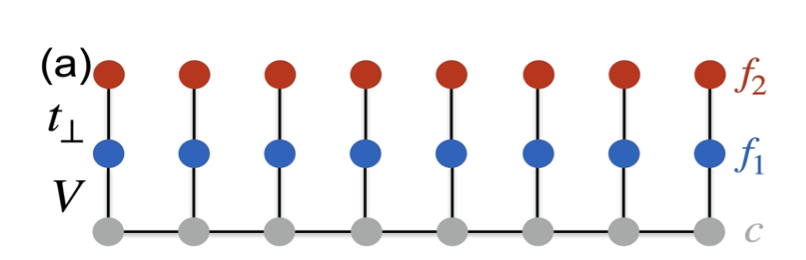
\includegraphics[scale=0.8]{/mnt/d/共享文件夹/毕设论文/latex模板/figures/figure10.png}
    \caption{晶格几何的一维表示,包括c,$f_1$。}
    \label{fig4.1.3}
\end{figure}

\subsection{行列式量子蒙特卡洛(DQMC)}%蒙特卡洛
\subsubsection{蒙特卡洛}
蒙特卡罗方法,也称统计模拟方法,是1940年代中期由于科学技术的发展和电子计算机的发明,而提出的一种以概率统计理论为指导的数值计算方法。是指使用随机数(或更常见的伪随机数)来解决很多计算问题的方法。

对于稳态分布$\pi(i)$,我们有细致平衡条件:
$$
\pi(i)Q(i,j)\alpha(i,j)=\pi(j)Q(j,i)\alpha(j,i)
$$
其中$Q(i,j)$表示从$i$尝试跳往$j$的概率,$\alpha(i,j)$为相应的接收的概率。我们通常选择:
$$
\alpha(i,j)=min\left \{\frac{\pi(j)Q(j,i)}{\pi{i}Q(i,j)},1\right \}
$$
\\大多数情况下$Q(i,j)=Q(j,i)$。如经典Ising模型的Metropolis中,每个构型的权重$\propto e^{-\beta E}$,接收概率为$min \left \{ e^{-\beta \Delta E},1 \right \}$
\subsubsection{统计}
对于经典模型,我们有配分函数:
$$
Z=\sum_\sigma e^{-\beta E_\sigma}
$$

物理量:
$$
\left \langle O \right \rangle=\frac{1}{Z} \sum_C O e^{-\beta E_C}
$$

对于量子系统,配分函数:
$$
Z=Tr\{e^{-\beta H}\}
$$

选一组basis:
$$
Z=\sum_{\{\phi \}} \left \langle \{\phi \} | e^{-\beta H}| \{\phi \} \right \rangle
$$

物理量:
$$
\left \langle O \right \rangle=\frac{Tr\{ O e^{-\beta H} \}}{Z}
$$


\subsubsection{量子蒙特卡洛}
DQMC模拟强关联系统的强有力的工具。强关联系统意味着量子粒子(例如电子)无法用独立电子近似描述(类似于密度泛函理论和能带结构计算)。

DQMC主要用来计算有限温度的费米子系统。DQMC将求Trace转化为了求矩阵的行列式。例如:
$$Tr[e^{- \sum_{i,j}\widehat{c}^\dagger_i A_{i,j}\widehat{c}_j}]=Det[\textbf{1}+e^{-\textbf{A}}]$$
其中$A_{i,j}$为矩阵A的元素,可以看到将求Trace转为求一个单位矩阵\textbf{1}加上矩阵$e^{-\textbf{A}}$。
对于此证明,将e指数上的部分进行对角化,Trace即为对于$n_i=0,1$的可能性求和:
$$
\operatorname{Tr}\left[e^{-\sum_{i, j} \hat{c}_{i}^{\dagger} A_{i, j} \hat{c}_{j}}\right]=\operatorname{Tr}\left[e^{-\sum_{k} \epsilon(k) \hat{c}_{k}^{\dagger} \hat{c}_{k}}\right]=\Pi_{k} \operatorname{Tr}\left[e^{-\epsilon(k) \hat{c}_{k}^{\dagger} \hat{c}_{k}}\right]=\Pi_{k}\left[1+e^{-\epsilon(k)}\right]
$$
上述等式显然成立。
对于上式推广:
$$
e^{-\sum_{i, j} c_{i}^{\dagger} A_{i, j} c_{j}} e^{-\sum_{i, j} c_{i}^{\dagger} B_{i, j} c_{j}}=e^{-\sum_{\nu} c_{\nu}^{\dagger} l_{\nu} c_{\nu}}
$$
从单粒子态开始:$e^{-A}e^{-B}$的作用在$|\psi \rangle=c^{\dagger}_v|0\rangle$:
$$
e^{-\sum_{i, j} c_{i}^{\dagger} A_{i, j} c_{j}} e^{-\sum_{i, j} c_{i}^{\dagger} B_{i, j} c_{j}}|\psi\rangle=\left(e^{-A} e^{-B}\right)_{\nu \nu} c_{\nu}^{\dagger}|0\rangle=e^{-l_{\nu}} c_{\nu}^{\dagger}|0\rangle
$$

考虑一个多粒子态比如二粒子态$|\phi\rangle=c^\dagger _{\mu_1}c^\dagger _{\mu_2}|0\rangle$,有:
$$
\begin{aligned}
e^{-c_{i}^{\dagger} B_{i j} c_{j}}|\phi\rangle &=\prod_{\mu}\left[1+\left(e^{-B_{\mu}}-1\right) c_{\mu}^{\dagger} c_{\mu}\right] c_{\mu_{1}}^{\dagger} c_{\mu_{2}}^{\dagger}|0\rangle \\
&=e^{-B_{\mu_{1}}} e^{-B_{\mu_{2}}} c_{\mu_{1}}^{\dagger} c_{\mu_{2}}^{\dagger}|0\rangle
\end{aligned}
$$
因此有:
$$
\operatorname{Tr}\left[e^{-\sum_{i, j} c_{i}^{\dagger} A_{i, j} c_{j}} e^{-\sum_{i, j} c_{i}^{\dagger} B_{i, j} c_{j}}\right]=\operatorname{Det}\left(1+e^{-\mathbf{A}} e^{-\mathbf{B}}\right)
$$

本论文着重于对DQMC产生的数据进行分析,以及相关程序的编写。
\subsection{分析程序}
%哈密顿量
由于我们计算结果都存放在远程服务器上,而我们需要在本地备份数据并且输出结果,所以我们在本地编写数据处理程序来帮助我们处理数据。
\subsubsection{运行所需环境}
我们的编写环境在Macos以及Linux下,程序语言是python,如下是需要的运行python库,其中pexpect库无法在Windows环境下运行,需要安装WSL2。
\begin{lstlisting}
    import pexpect
    from pathlib import Path
    import os
    import matplotlib.pyplot as plt
    import re
\end{lstlisting}

\subsubsection{程序编写思路}
我们将数据从服务器下载到本地处理,利用pexpect库向终端提交scp命令将数据打包下载到本地处理\cite{}。
\begin{lstlisting}
    cmdline = 'scp -r %s %s@%s:%s' % (filename, user, ip, dst_path)
\end{lstlisting}
接着我们定义了四个函数利用字符串格式化匹配数据文件名
\begin{lstlisting}
def filename_U4(self, V1_value, V2s_value, Nsite, seed, T, mus):
    return "U4_V{}_tp{}_N{}_be{}_{}_mu{}.out".format(V1_value, V2s_value, Nsite, T, seed, mus)

def filename_local_orb(self, V1_value, V2s_value, Nsite, seed,T,mus):
    return "local_orb_U4_V{}_tp{}_N{}_be{}_{}_mu{}".format(V1_value, V2s_value, Nsite, T,seed, mus)

def filename_U4_tdm(self, V1_value, V2s_value, Nsite, seed,T, mus):
    return "U4_V{}_tp{}_N{}_be{}_{}_mu{}.tdm.out".format(V1_value, V2s_value, Nsite,T,seed, mus)

def filename_geom(self,V1_value,V2s_value,Nsite):
    return "geomU4_V{}_tp{}_N{}".format(V1_value,V2s_value,Nsite)
\end{lstlisting}
在获取文件名后利用python读取文件数据,进行字符串匹配,例如输出对.out文件的数据输出如下,返回数据存放在列表中。
\begin{lstlisting}
def data_out(self, path,filename, strs, numstart, numend):#输出结果
    data_list=[]
    a=[]
    b=[]
    with open(filename, 'r') as f:
        for i in f.readlines():
            data_list.append(i)
    for i in range(numstart,numend):
            k =data_list[i]
            result = "".join(k.split())
            a.append(result)
    for j in range(len(a)):
        if strs in a[j]:
            data_analysis.data_write(self,path,'result',data_list[j+numstart])
            b.append(data_list[j+numstart])
    return b
\end{lstlisting}
最后如下所示代码通过matplotlib库以及通过正则表达式对数据进行整合输出成图表,并且由于是面对对象的编程,本程序完成编写后可以为其他的程序调用,减轻了数据处理的负担。
\begin{lstlisting}
def data_temperature(self,path,ls,dtaus,V1_value,V2s_value,Nstie,\\ seed,mus,file):
    b=[]
    x=[]
    l=[]
    y=[]
    y0=[]
    err=[]
    y0err=[]
    for i in range(len(ls)):
        b.append(ls[i]*dtaus[i])
        x.append(1/(ls[i]*dtaus[i]))
    path1 = data_analysis.mkdir(self, path, V1_value, V2s_value, Nsite,mus)  # 创建文件夹返回路径
    path3 = path1 + '/' + file
    for k in b:
        filename_tdm=data_analysis.filename_U4_tdm(self,V1_value,V2s_value,\\ Nsite,seed,k,mus)
        if data_analysis.exit(self,path3,filename_tdm)==True:
            print('exit',filename_tdm)
        else:
            print("don't exit:",filename_tdm)
            data_analysis.download(self, '10.10.8.74', 'zhumo', '/home/zhumo/run_Ce3PtIn11/test', path1)
        l.append(data_analysis.data_tdm_out(self,path3,path3+'/'+
        filename_tdm,'Pd'))
    for i in l:
        p=re.findall(r"\d+\.?\d*",i[0])
        negative_p=re.findall(r"-\d+\.?\d*",i[0])
        print(p,negative_p)
        y.append(float(p[2])*10**float(p[3]))
        err.append(float(p[4])*10**float(negative_p[0]))
        y0.append(float(p[6])*10**float(p[7]))
        y0err.append(float(p[8])*10**float(negative_p[1]))
    plt.figure()
    plt.errorbar(x,y,yerr=err,fmt='-co')
    plt.errorbar(x,y0,yerr=y0err,fmt=',',ecolor='b',capsize=3)
    plt.xlabel('T')
    plt.ylabel('Pd_Pd0')
    plt.title(str(V1_value)+'-'+str(V2s_value),fontsize=12)
    plt.legend(title=('Pd','Pd0'))
    plt.ylim(0,0.5)
    # plt.xlim(0,30)
    plt.show()
\end{lstlisting}



\subsection{反铁磁结构因子}%定义
我们计算$f$轨道的反铁磁结构因子(AF),
$$
S_{\mathrm{AF}}^{f}\left(V_{1}, V_{2}\right)=\frac{1}{N} \sum_{i j} e^{-i \mathbf{q} \cdot\left(\mathbf{R}_{\mathbf{i}}-\mathbf{R}_{\mathbf{j}}\right)}\left\langle\left(n_{i \uparrow}^{f}-n_{i \downarrow}^{f}\right)\left(n_{j \uparrow}^{f}-n_{j \downarrow}^{f}\right)\right),
$$
其中$\mathbf{q}=(\pi,\pi)$,$\mathbf{R_i}$表示位点$j$的坐标,$N$表示晶格大小。

为了对模型进行测试。与之前发表文章中的图\ref{fig5}(b)进行比对。其中参数如下:$V_1=1.0$、$V_{2s}=1.0$、$V_{12s}=0.005$,晶格大小为$N=6 \times 6$,


% \begin{figure}[htbp]
%     \centering
%     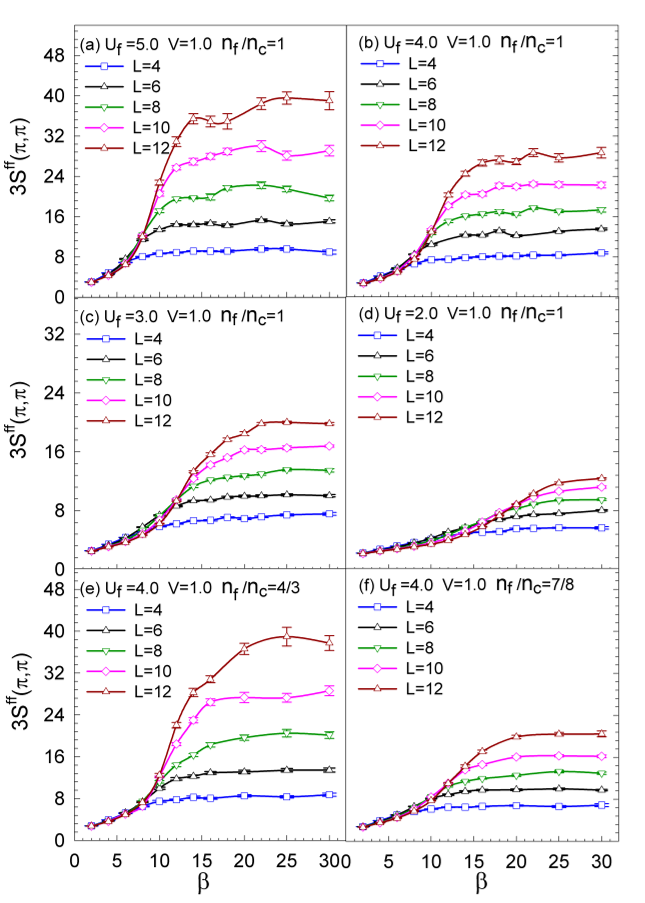
\includegraphics[scale=0.5]{/mnt/d/共享文件夹/毕设论文/latex模板/figures/figure3.png}
%     \caption{(a)-(d)展示了在V=1时随着$\beta$的增加以及不同晶格大小的情况下AF结构因子的变化\cite{10}。}
%     \label{fig5}
% \end{figure}


% \begin{figure}[h]
%     \centering
%     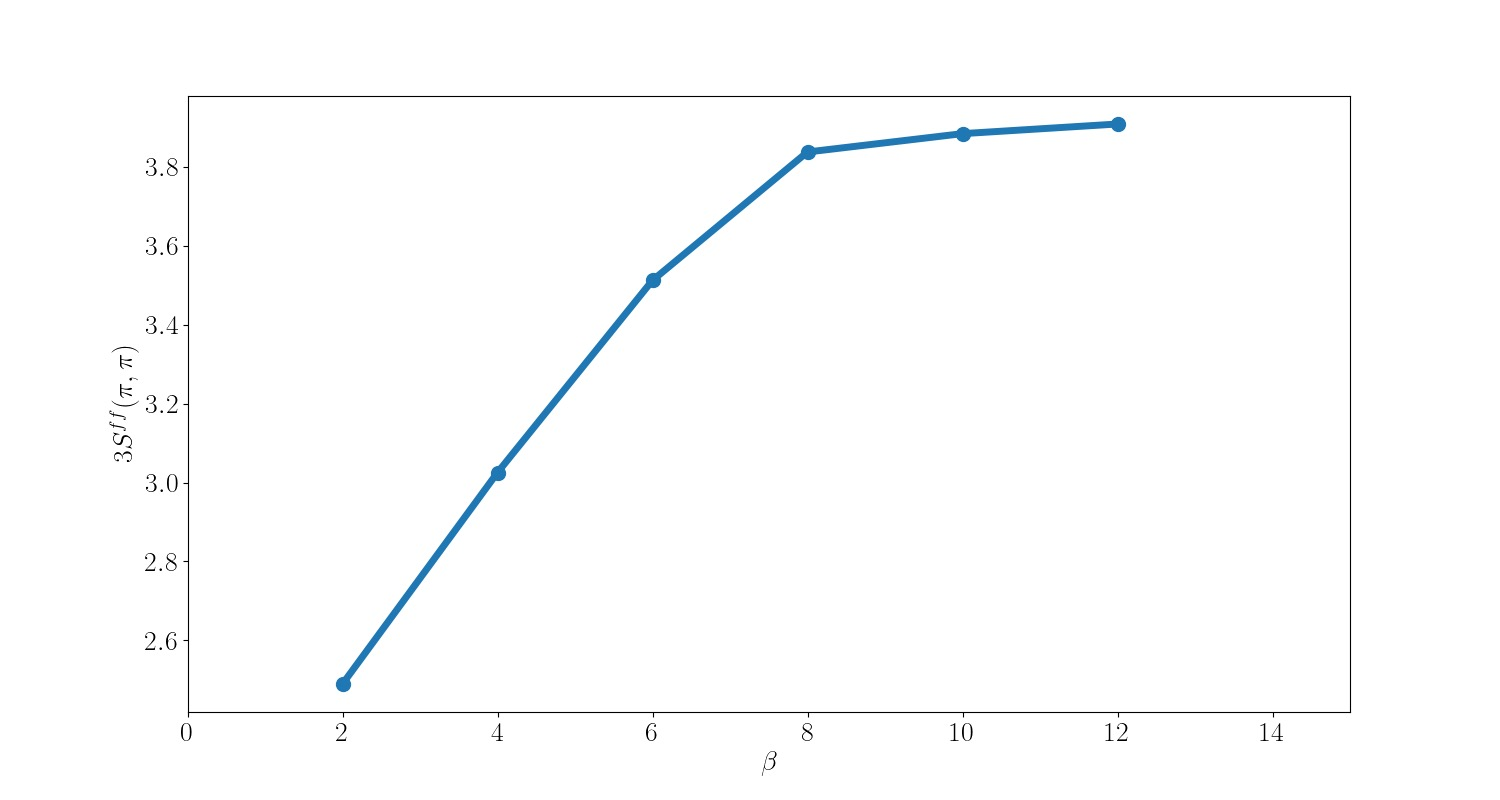
\includegraphics[scale=0.25]{/mnt/d/共享文件夹/毕设论文/latex模板/figures/figure7.png}
%     \caption{横坐标$\beta=1/T$,而纵坐标为反铁磁结构因子。其中由于时间关系本文只计算了$N=6$,温度$T=0.5t,0.25t,0.167t,0.125t,0.1t,0.083 t$。}
%     \label{fig7}
% \end{figure}

\begin{figure}
    \centering
    \subfigure{ 
    \begin{minipage}[b]{0.7\textwidth}
        \centering   
    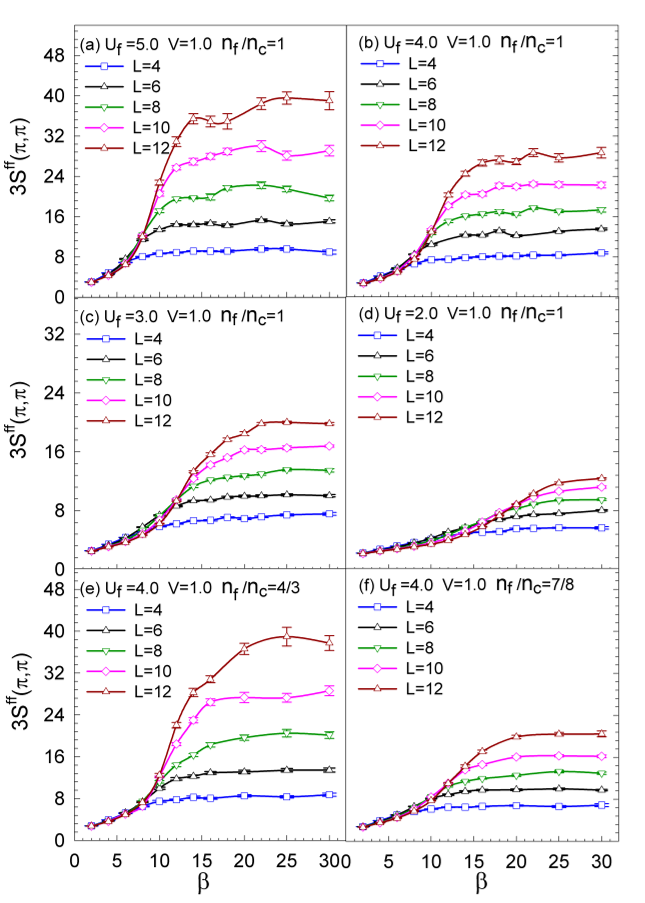
\includegraphics[width=1\textwidth]{/mnt/d/共享文件夹/毕设论文/latex模板/figures/figure3.png}  
    \caption{在V=1时随着$\beta$的增加以及不同晶格大小的情况下AF结构因子的变化\cite{10}。}
    \label{fig5} 
    \end{minipage}   
    }    
    \subfigure{   
    \begin{minipage}[b]{0.7\textwidth}   
    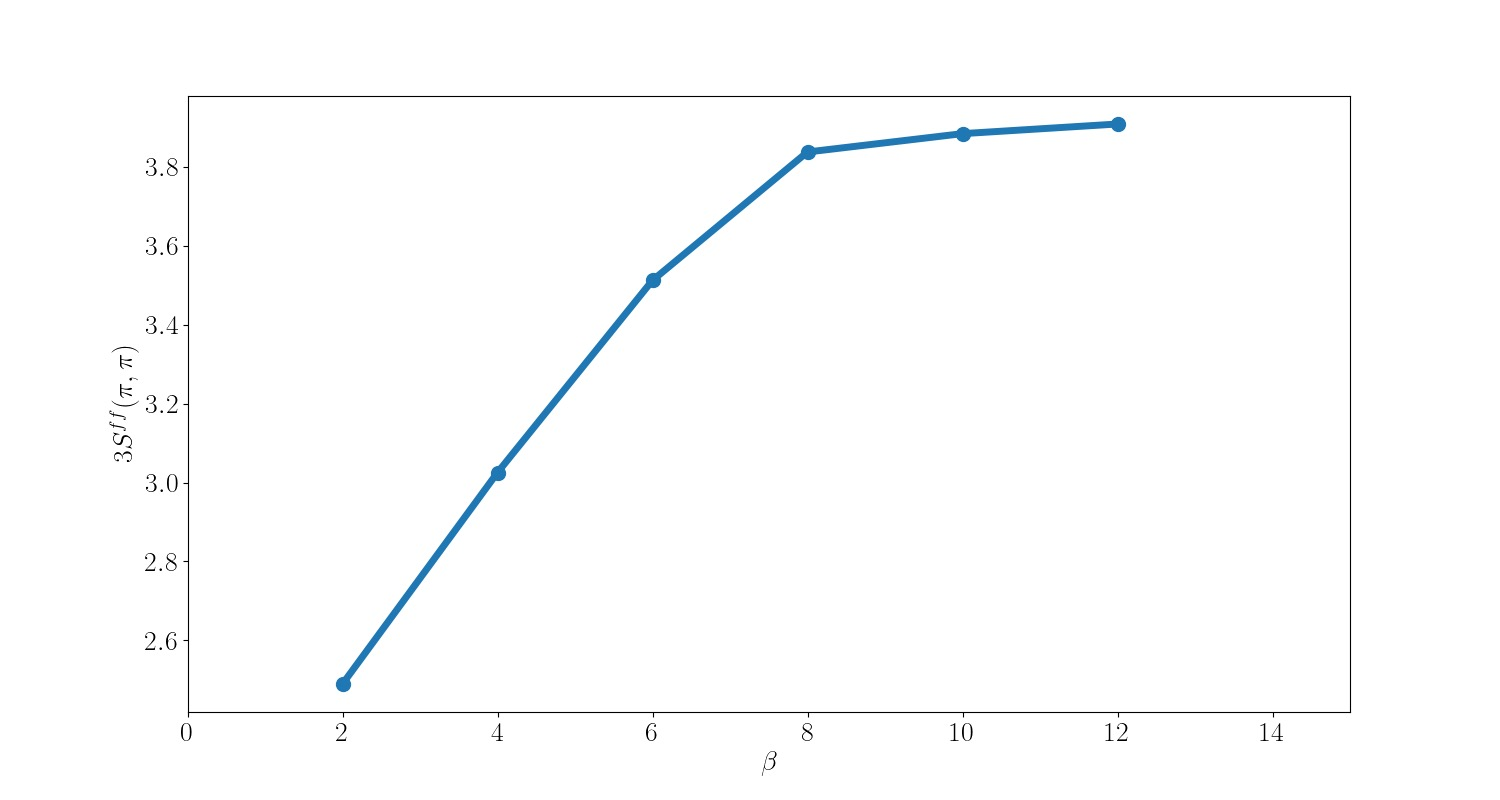
\includegraphics[width=1\textwidth]{/mnt/d/共享文件夹/毕设论文/latex模板/figures/figure7.png} 
    \caption{横坐标$\beta=1/T$,而纵坐标为反铁磁结构因子。计算的温度为$T=0.5t,0.25t,0.167t,0.125t,0.1t,0.083 t$。} 
    \label{fig7}  
    \end{minipage}
        } 
    \end{figure}
    
其中V1\_value是图\ref{fig4.1.1}中的$V_1$,同理V2s\_value是图\ref{fig4.1.1}中的$V_2$。通过服务器的模拟结果如图\ref{fig7}所示。与文献中符合的较好。


\subsection{d波超导}
Hubbard模型有掺杂之后,会出现d波超导,类似的我们构建的模型掺杂之后,也可能会出现d波超导。因此,通过计算$f$电子的d波配对磁化率来研d波超导电性,
\begin{equation}
    \begin{aligned}
    P_{d}=& \frac{1}{N} \frac{1}{G} \sum_{i j} \sum_{\delta \delta^{\prime}} g\left(\delta^{\prime}\right) g^{*}(\delta) \\
    & \times \int_{0}^{\beta}\left\langle f_{j+\delta^{\prime}, \downarrow}(\tau) f_{j, \uparrow}(\tau) f_{i, \uparrow}^{\dagger}(0) f_{i+\delta, \downarrow}^{\dagger}(0)\right\rangle d \tau
    \label{4.5}
    \end{aligned}
\end{equation}
其中$g(\delta)$是实空间的一般形状因子,$G=\sum_\delta |g(\delta)|^2$是归一化因子。特别的,对于d波配对通道,沿x和y方向的最近邻分离$\delta$的$g(\delta)=\pm 1$。相似的我们可以定义和计算无顶点修正的磁化率$P^0_d$。在DQMC模拟中,$P_d$和$P^0_d$的区别在于计算公式\ref{4.5}中的四费米的期望值。准确的说,$P_d(p^0_d)$包含由Wick缩并得到的格林函数,先相乘(平均),然后再平均(相乘)。因此,$P_d$包含所有相互作用影响,而$P^0_d$仅考虑单粒子水平的相互作用。我们可以进一步定义交互顶点
\begin{equation}
    \Gamma_d=\frac{1}{P_d}-\frac{1}{p^0_d}
    \label{4.2}
\end{equation}
所以$\Gamma_d P^0_d$的符号反映配对相互作用是排斥(正)还是吸引(负)。方程\ref{4.2}可以被改写成
\begin{equation}
    P_d=\frac{P^0_d}{1+\Gamma_d P^0_d}
\end{equation}
所以$\Gamma_d P^0_d=-1$标志着d波超导的产生。

利用DQMC计算二维Hubbard模型的超导相,以下是设置参数:
为了对模型进行测试。与之前发表文章中的图\ref{fig5}(b)进行比对。其中参数如下:

$V_1=1.0$、$V_{2s}=0.001$、$V_{12s}=0.001$,晶格大小为$N=4 \times 4$,计算的温度为$T=0.125t, 0.167t, 0.25t, 0.33t$。

\begin{figure}[H]
    \centering
    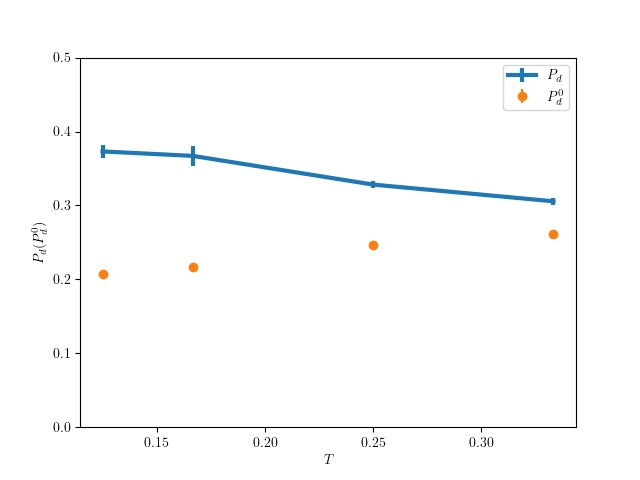
\includegraphics[scale=0.42]{/mnt/d/共享文件夹/毕设论文/latex模板/figures/figure9.png}
    \caption{$P_d$和$P_d^0$随温度的变化}
    \label{fig9}
\end{figure}

\begin{figure}[H]
    \centering
    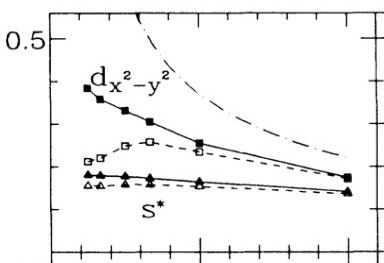
\includegraphics[scale=0.7]{/mnt/d/共享文件夹/毕设论文/latex模板/figures/figure8.jpg}
    \caption{在半填充($\left \langle n \right \rangle=1$)下,绘制了不同对场模式下对场磁化率P(实心点)和不相关对场磁化率P(空心点)与T的关系图\cite{11}。}
    \label{fig8}
\end{figure}

利用图\ref{fig8}验证结果正确性,计算结果如图\ref{fig9}所示。


























